\chapter{GUIDE en Matlab} \cite{ML} \cite{MML}

\textbf{GUIDE}  son las siglas en ingles de “Graphic User Interfaze Development Environment”. Es un entorno de desarrollo de interfaces gráficas de usuario que proporciona MATLAB para facilitar la inserción de datos en aplicaciones por parte de los usuarios.
\bigskip

Esta herramienta se encarga de generar el código necesario para la creación de interfaces gráficas diseñadas en un entorno gráfico sin necesidad de una programación completa de las mismas, facilitando al programador el trabajo, que ya desarrolla el código vinculado a los eventos que se produzcan en la GUI.

\section{Componentes del entorno}

Para abrir el entorno en la consola de MATLAB se ejecuta el comando “guide” que muestra la pantalla de la figura 6.1.

\begin{figure}
\centering
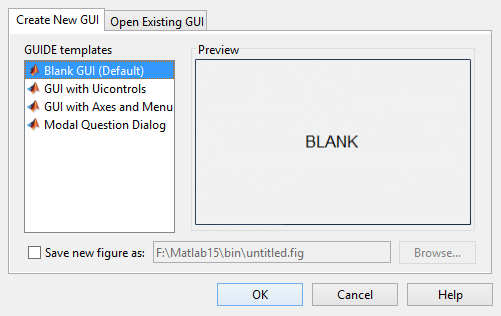
\includegraphics[width=0.9\textwidth]{imagenes/figuras/6_1.png}
\caption{Ventana incio GUIDE.}
\end{figure}

Las opciones que nos muestra son:

\begin{itemize}
\item \textbf{Blank GUI} crea una nueva interfaz en blanco para agregar los elementos que se deseen.
\item \textbf{GUI with UIcontrols} muestra un ejemplo de utilización de los controles de interfaz de usuario.
\item \textbf{GUI with Axes and Menu} muestra un ejemplo de interfaz con un menú desplegable para seleccionar un tipo de gráfico que se mostrará en el elemento Axes, que es un elemento de la GUI que sirve para proyectar gráficos de distintos tipos.
\item \textbf{Modal Question Dialog} muestra un ejemplo de interfaz con una pregunta que se puede responder con un sí o un no y según el botón pulsado devuelve una cosa u otra.
\end{itemize}

La opción más usual es Blank GUI para diseñar la interfaz deseada, mientras que las otras pueden servir de ejemplo para iniciarse en GUIDE. Una vez seleccionada dicha opción nos aparece la siguiente interfaz:


\begin{figure}[H]
\centering
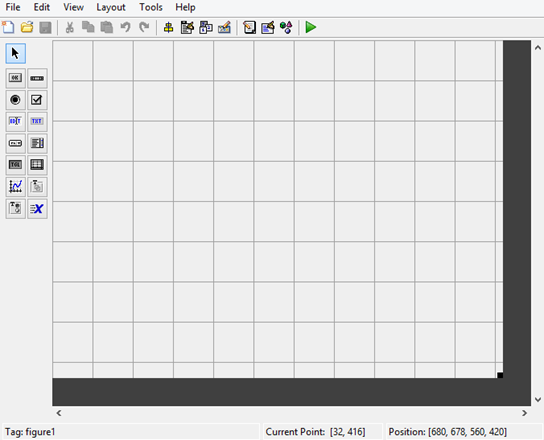
\includegraphics[width=0.9\textwidth]{imagenes/figuras/6_2.png}
\caption{GUIDE Blank GUI}
\end{figure}
\bigskip

Los elementos gráficos disponibles en GUIDE son:

\begin{table}[htb]
\begin{center}
\resizebox{10cm}{!} {
\begin{tabular}{|l|c|l|}
\hline
Elemento & Icono & Descripción \\
\hline \hline
Push Button&  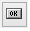
\includegraphics[width=0.05\textwidth]{imagenes/iconosguide/pushbuton.png} & Botón de una sola posición \\ \hline
Slider &
\includegraphics{imagenes/iconosguide/slider.png} & Barra deslizante \\ \hline
Radio Button&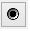
\includegraphics{imagenes/iconosguide/radiobuton.png}  &Botón de selección única \\ \hline
Check Box&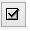
\includegraphics{imagenes/iconosguide/check.png}   &Caaja de selección o botón de selección múltiple\\ \hline
Edit Text & 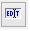
\includegraphics{imagenes/iconosguide/edit.png} &Caja de texto editable  \\ \hline
Static Text& 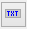
\includegraphics{imagenes/iconosguide/text.png} &Caja de texto no modificable  \\ \hline
Pop-up Menu& 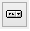
\includegraphics{imagenes/iconosguide/popup.png}  & Menú de selección desplegable\\ \hline
List Box&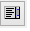
\includegraphics{imagenes/iconosguide/list.png}  &Lista delementos seleccionable \\ \hline
Toggle Button& 
\includegraphics{imagenes/iconosguide/togle.png}  &Botón de dos posiciones\\ \hline
Table&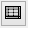
\includegraphics{imagenes/iconosguide/table.png}   &Tabla numerada en filas y columnas\\ \hline
Axes&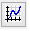
\includegraphics{imagenes/iconosguide/axes.png}   &Elemento para inserción de gráficos\\ \hline
Panel&
\includegraphics{imagenes/iconosguide/panel.png}  & Contenedor que puede reunir uno o varios elementos  \\ \hline
Button Group&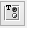
\includegraphics{imagenes/iconosguide/butongroup.png}   &Contenedor que agrupa Radio Buttons\\ \hline
ActiveX control&
\includegraphics{imagenes/iconosguide/activex.png}   &Contenedor de elementos ActiveX\\ \hline
\end{tabular}
}
\caption{Elementos de la interfaz gráfica.}
\end{center}
\end{table}
\bigskip

Cada uno de los elementos tiene una serie de propiedades modificables mediante el “property inspector”. Las propiedades más comunes a todos los elementos son el nombre (Tag), la posición en la que se encuentra dentro de la interfaz (Position), si está activo o no, si es visible o no y algunas relacionadas con el formato y tipo de fuente así como con la estética del elemento. En la figura 6.3 podemos ver un ejemplo de property inspector.
\bigskip

\begin{figure}
\centering
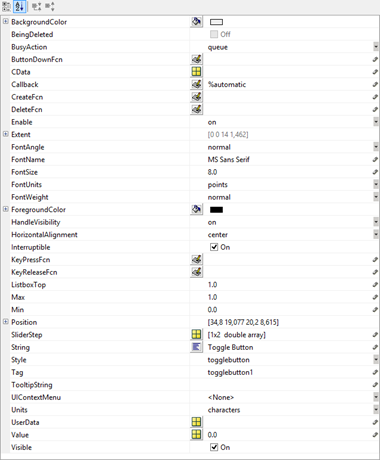
\includegraphics[width=0.6\textwidth]{imagenes/figuras/6_3.png}
\caption{Property Inspector.}
\end{figure}

Las demás propiedades son relativas al funcionamiento de cada elemento y no son comunes.
\bigskip

Otras opciones disponibles en GUIDE son las mostradas en la barra de herramientas(Tabla 6.2).

\begin{table}[H]
\begin{center}
\resizebox{12cm}{!} {
\begin{tabular}{|l|c|l|}
\hline
Herramienta & Icono & Descripción \\
\hline \hline
Nuevo&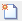
\includegraphics{imagenes/iconosguide/nuevo.png} & Abre la ventana guide para crear nuevas interfaces \\ \hline
Abrir &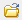
\includegraphics{imagenes/iconosguide/abrir.png} & Abre una interfaz anteriormente guardada \\ \hline
Guardar &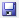
\includegraphics{imagenes/iconosguide/guardar.png} &Guarda la interfaz actual \\ \hline
Cortar&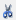
\includegraphics{imagenes/iconosguide/cortar.png}  &Corta el elemento seleccionado\\ \hline
Copiar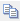
\includegraphics{imagenes/iconosguide/copiar.png} & &Copia el elemento seleccionado\\ \hline
Pegar&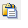
\includegraphics{imagenes/iconosguide/pegar.png} &Pega un elemento previamente cortado o copiado  \\ \hline
Atrás&
\includegraphics{imagenes/iconosguide/atras.png}  & Elimina el último cambio realizado en la interfaz\\ \hline
Adelante&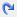
\includegraphics{imagenes/iconosguide/adelante.png} &Repone el paso previamente eliminado \\ \hline
Alinear&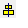
\includegraphics{imagenes/iconosguide/align.png}  &Abre un menú en el que se muestran distintos métodos de alineamiento de elementos del interfaz\\ \hline
Editor de menús &
\includegraphics{imagenes/iconosguide/menueditor.png} &Abre un entorno para la creación de menús\\ \hline
Inspector de propiedades&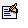
\includegraphics{imagenes/iconosguide/propert.png}  &Abre el inspector de propiedades\\ \hline
Editor de pestañas &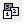
\includegraphics{imagenes/iconosguide/tabordereditor.png} &Abre una ventana para editar el orden de las distintas pestañas que tenga la interfaz\\ \hline
Editor de barras de herramientas&
\includegraphics{imagenes/iconosguide/toolbareditor.png} &Abre un editor para la creación de barras de herramientas en la interfaz  \\ \hline
Editor&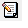
\includegraphics{imagenes/iconosguide/editor.png}  & Abre el código del elemento marcado\\ \hline
Buscador de objetos&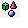
\includegraphics{imagenes/iconosguide/object.png} &Muestra todos los elementos que maneja la interfaz para buscar uno en concreto \\ \hline
Run&
\includegraphics{imagenes/iconosguide/run.png}  & Arranca la interfaz en modo ejecución\\ \hline
\end{tabular}
}
\caption{Herramientas disponibles en GUIDE.}
\end{center}
\end{table}
\bigskip

Una vez creada una nueva interfaz al darle a guardar genera dos ficheros uno de ellos “.fig” en el que se almacena los elementos gráficos del diseño y otro “.m” donde se inserta el código necesario para que funcione la misma.
\bigskip

Es dentro del fichero “.m” donde se tiene que añadir el código necesario para el funcionamiento de la aplicación. En dicho fichero insertaremos el código de los eventos de cada uno de los elementos de la interfaz, que en GUIDE se llaman “callbacks” y se añaden haciendo click con el botón derecho del ratón sobre el elemento concreto y en el menú desplegado pulsando en “View Callbacks” se muestran los distintos eventos que puede manejar el elemento seleccionado.
\bigskip

\section{Manejo desde código}

Para manejar cada uno de los elementos desde el código se utiliza el objeto hObject que se incluye como argumento de cada una de las llamadas a los métodos “callback” entre otros.
\bigskip

Dicho objeto sirve de contenedor, y para modificar cualquier dato se asigna a “handles” de la siguiente forma:
\bigskip

\textbf{handles.output = hObject;} 
\bigskip

Por ejemplo para tomar un elemento del interfaz gráfico se puede hacer:

\bigskip

\textbf{campo\_texto=get(handles.text1,’String’);}
\bigskip

Esto almacena en la variable campo\_texto el valor (Value) que tenga el campo de texto text1, para modificar el valor del mismo en el interfaz se debe  hacer con “set”:
\bigskip

\textbf{set(handles.text1,’String’, ‘Nuevo valor’);}
\bigskip

Con esta última sentencia se mostrara el texto “Nuevo valor” en el campo de texto text1 del interfaz.
\bigskip

En el caso de querer tomar los valores de “RadioButtons”, “Checkboxes”, “Lists”, etc, se tiene que hacer un get pero con el parámetro “Value” en lugar del “String”:
\bigskip

\textbf{Valor = get(handles.radio1,’Value’)}
\bigskip

La sentencia anterior devolverá 0 o 1 dependiendo si está o no marcado el radioButton radio1. Si en lugar de este tipo de elemento se tuviera una lista, ya sea desplegable o con slider, lo que devolvería “Value” seria la posición del elemento seleccionado de la lista.
\bigskip

\section{Ejemplo sencillo de interfaz con GUIDE}

En este apartado se va a mostrar un ejemplo sencillo de interfaz gráfica que mostrará un texto dentro de un campo de texto cuando se pulse un botón, el aspecto de la interfaz es:
\bigskip

\begin{figure}[H]
\centering
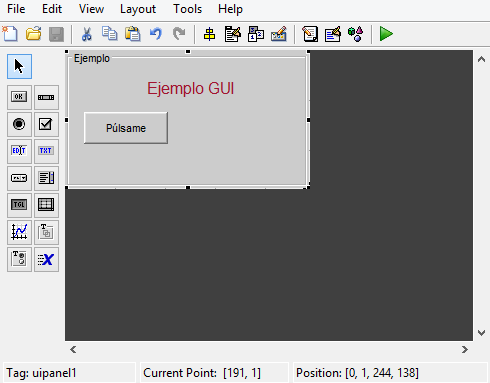
\includegraphics[width=0.9\textwidth]{imagenes/figuras/6_4.png}
\caption{Ejemplo de GUI, vista en GUIDE.}
\end{figure}
\bigskip

Esta es la vista desde GUIDE, la vista en ejecución es:
\bigskip

\begin{figure}[H]
\centering
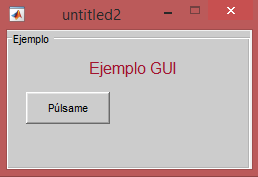
\includegraphics[width=0.9\textwidth]{imagenes/figuras/6_5.png}
\caption{Ejemplo GUI, vista en ejecución.}
\end{figure}
\bigskip

La última vista es tras pulsar el botón:
\bigskip

\begin{figure}[H]
\centering
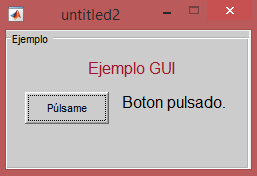
\includegraphics[width=0.9\textwidth]{imagenes/figuras/6_6.png}
\caption{Ejemplo GUI, vista tras pulsar el botón.}
\end{figure}
\bigskip

El código asociado al callback del botón es:
\bigskip

\begin{figure}[H]
\centering
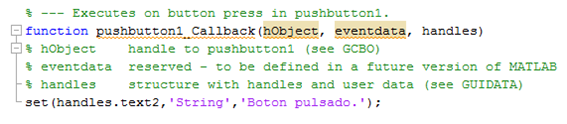
\includegraphics[width=0.9\textwidth]{imagenes/figuras/6_7.png}
\caption{Código del callback.}
\end{figure}
\bigskip

Para un ejemplo más complejo del manejo de la interfaz desde el código ver el capítulo “implementación”.